% questions.tex —— 2011 年·湖北卷·理科 · 题目内容片段（无答案）
% 由 tools/generate_projects.py 依来源总账自 2011/2011_数学真题_湖北理_试题.md 生成，勿手改（改源 MD 后重跑）

\gkpart{一、选择题}

\begin{question}
\gkti{1}$\mathrm i$ 为虚数单位，则 $\left(\dfrac{1+\mathrm i}{1-\mathrm i}\right)^{2011}=$\mbox{（　　）}

（A）$-\mathrm i$

（B）$-1$

（C）$\mathrm i$

（D）$1$

\end{question}
\begin{question}
\gkti{2}已知 $U=\{y\mid y=\log_2x,\ x>1\}$，$P=\left\{y\ \middle|\ y=\dfrac1x,\ x>2\right\}$，则 $\complement_UP=$\mbox{（　　）}

（A）$\left[\dfrac12,+\infty\right)$

（B）$\left(0,\dfrac12\right)$

（C）$(0,+\infty)$

（D）$(-\infty,0)\cup\left[\dfrac12,+\infty\right)$

\end{question}
\begin{question}
\gkti{3}已知函数 $f(x)=\sqrt3\sin x-\cos x$，$x\in\mathbf R$。若 $f(x)\geqslant1$，则 $x$ 的取值范围为\mbox{（　　）}

（A）$\left\{x\ \middle|\ k\pi+\dfrac\pi3\leqslant x\leqslant k\pi+\pi,\ k\in\mathbf Z\right\}$

（B）$\left\{x\ \middle|\ 2k\pi+\dfrac\pi3\leqslant x\leqslant2k\pi+\pi,\ k\in\mathbf Z\right\}$

（C）$\left\{x\ \middle|\ k\pi+\dfrac\pi6\leqslant x\leqslant k\pi+\dfrac{5\pi}6,\ k\in\mathbf Z\right\}$

（D）$\left\{x\ \middle|\ 2k\pi+\dfrac\pi6\leqslant x\leqslant2k\pi+\dfrac{5\pi}6,\ k\in\mathbf Z\right\}$

\end{question}
\begin{question}
\gkti{4}将两个顶点在抛物线 $y^2=2px$（$p>0$）上，另一个顶点是此抛物线焦点的正三角形个数记为 $n$，则\mbox{（　　）}

（A）$n=0$

（B）$n=1$

（C）$n=2$

（D）$n\geqslant3$

\end{question}
\begin{question}
\gkti{5}已知随机变量 $\xi$ 服从正态分布 $N(2,\sigma^2)$，且 $P(\xi<4)=0.8$，则 $P(0<\xi<2)=$\mbox{（　　）}

（A）$0.6$

（B）$0.4$

（C）$0.3$

（D）$0.2$

\end{question}
\begin{question}
\gkti{6}已知定义在 $\mathbf R$ 上的奇函数 $f(x)$ 和偶函数 $g(x)$ 满足 $f(x)+g(x)=a^x-a^{-x}+2$（$a>0$，且 $a\neq1$）。若 $g(2)=a$，则 $f(2)=$\mbox{（　　）}

（A）$2$

（B）$\dfrac{15}4$

（C）$\dfrac{17}4$

（D）$a^2$

\Needspace{0.4\textheight}
\end{question}
\begin{question}
\gkti{7}如图，用 $K$、$A_1$、$A_2$ 三类不同的元件连接成一个系统。当 $K$ 正常工作且 $A_1$、$A_2$ 至少有一个正常工作时，系统正常工作。已知 $K$、$A_1$、$A_2$ 正常工作的概率依次为 $0.9$、$0.8$、$0.8$，则系统正常工作的概率为\mbox{（　　）}

（A）$0.960$

（B）$0.864$

（C）$0.720$

（D）$0.576$
\nopagebreak[4]
\begin{center}% 2011 年湖北卷理科第 7 题：K 与并联的 A1、A2 组成的系统。
% 来源 PDF：普通高考/2011/2011湖北理.pdf，SHA-256 ba721f03ae90f88887c5cde27ae98dbea165d33c73e5ba45b4e4f56b0638b075。
% 原页：第 1 页第 1 栏上部，书页码 667。
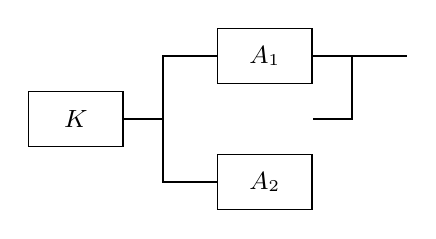
\begin{tikzpicture}[>=stealth, semithick, font=\small]
  \node[draw, minimum width=1.2cm, minimum height=0.7cm] (K) at (0,0) {$K$};
  \node[draw, minimum width=1.2cm, minimum height=0.7cm] (A1) at (2.4,0.8) {$A_1$};
  \node[draw, minimum width=1.2cm, minimum height=0.7cm] (A2) at (2.4,-0.8) {$A_2$};
  \draw (K.east) -- ++(0.5,0) coordinate (x) -- ++(0,0.8) -- (A1.west);
  \draw (x) -- ++(0,-0.8) -- (A2.west);
  \draw (A1.east) -- ++(0.5,0) coordinate (y) -- ++(0,-0.8) -- ++(-0.5,0);
  \draw (y) -- ++(0.7,0);
\end{tikzpicture}
\end{center}
\nopagebreak[4]
\end{question}
\begin{question}
\gkti{8}已知向量 $\boldsymbol a=(x+z,3)$，$\boldsymbol b=(2,y-z)$，且 $\boldsymbol a\perp\boldsymbol b$。若 $x$，$y$ 满足不等式 $|x|+|y|\leqslant1$，则 $z$ 的取值范围为\mbox{（　　）}

（A）$[-2,2]$

（B）$[-2,3]$

（C）$[-3,2]$

（D）$[-3,3]$

\end{question}
\begin{question}
\gkti{9}若实数 $a$，$b$ 满足 $a\geqslant0$，$b\geqslant0$，且 $ab=0$，则称 $a$ 与 $b$ 互补。记 $\varphi(a,b)=\sqrt{a^2+b^2}-a-b$，那么 $\varphi(a,b)=0$ 是 $a$ 与 $b$ 互补的\mbox{（　　）}

（A）必要而不充分条件

（B）充分而不必要条件

（C）充要条件

（D）既不充分也不必要条件

\end{question}
\begin{question}
\gkti{10}放射性元素由于不断有原子放射出微粒子而变成其他元素，其含量不断减少，这种现象称为衰变。假设在放射性同位素铯 137 的衰变过程中，其含量 $M$（单位：太贝克）与时间 $t$（单位：年）满足函数关系：$M(t)=M_02^{-\frac t{30}}$，其中 $M_0$ 为 $t=0$ 时铯 137 的含量。已知 $t=30$ 时，铯 137 含量的变化率是 $-10\ln2$（太贝克/年），则 $M(60)=$\mbox{（　　）}

（A）$5$ 太贝克

（B）$75\ln2$ 太贝克

（C）$150\ln2$ 太贝克

（D）$150$ 太贝克

\end{question}
\gkpart{二、填空题}

\begin{question}
\gkti{11}$\left(x-\dfrac1{3\sqrt x}\right)^{18}$ 的展开式中含 $x^{15}$ 的项的系数为 $\underline{\qquad}$。（结果用数值表示）

\end{question}
\begin{question}
\gkti{12}在 $30$ 瓶饮料中，有 $3$ 瓶已过了保质期。从这 $30$ 瓶饮料中任取 $2$ 瓶，则至少取到 $1$ 瓶已过保质期饮料的概率为 $\underline{\qquad}$。（结果用最简分数表示）

\end{question}
\begin{question}
\gkti{13}《九章算术》“竹九节”问题：现有一根 $9$ 节的竹子，自上而下各节的容积成等差数列，上面 $4$ 节的容积共 $3$ 升，下面 $3$ 节的容积共 $4$ 升，则第 $5$ 节的容积为 $\underline{\qquad}$ 升。

\Needspace{0.4\textheight}
\end{question}
\begin{question}
\gkti{14}如图，直角坐标系 $xOy$ 所在的平面为 $\alpha$，直角坐标系 $x'Oy'$（其中 $y'$ 轴与 $y$ 轴重合）所在的平面为 $\beta$，$\angle xOx'=45^\circ$。

（1） 已知平面 $\beta$ 内有一点 $P'\left(2\sqrt2,2\right)$，则点 $P'$ 在平面 $\alpha$ 内的射影 $P$ 的坐标为 $\underline{\qquad}$。

（2） 已知平面 $\beta$ 内的曲线 $C'$ 的方程是 $\left(x'-\sqrt2\right)^2+2y'^2-2=0$，则曲线 $C'$ 在平面 $\alpha$ 内的射影 $C$ 的方程是 $\underline{\qquad}$。
\nopagebreak[4]
\begin{center}% 2011 年湖北卷理科第 14 题：平面 α 与 β 成 45°，点与曲线在 α 内的射影。
% 来源 PDF：普通高考/2011/2011湖北理.pdf，SHA-256 ba721f03ae90f88887c5cde27ae98dbea165d33c73e5ba45b4e4f56b0638b075。
% 原页：第 1 页第 2 栏中部，书页码 667。示意。
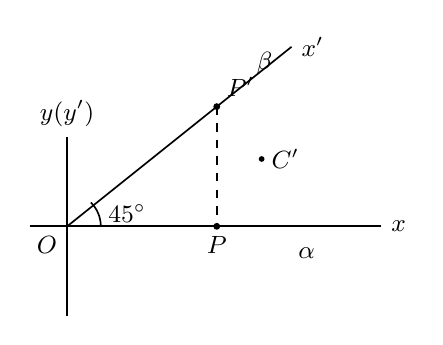
\begin{tikzpicture}[>=stealth, semithick, font=\small, scale=0.95]
  % α 平面（水平）
  \draw (-0.5,0) -- (4.2,0) node[right] {$x$};
  \draw (0,-1.2) -- (0,1.2) node[above] {$y(y')$};
  \node[below left] at (0,0) {$O$};
  \node[below] at (3.2,-0.15) {$\alpha$};
  % β 平面（斜向上 45°）
  \draw (0,0) -- (3.0,2.4) node[right] {$x'$};
  \node[above right] at (2.4,1.9) {$\beta$};
  \draw[dashed] (2.0,1.6) -- (2.0,0) node[below] {$P$};
  \fill (2.0,1.6) circle (1.3pt) node[above right] {$P'$};
  \fill (2.0,0) circle (1.3pt);
  \draw (0.45,0) arc (0:45:0.45) node[midway, right] {$45^\circ$};
  \fill (2.6,0.9) circle (1.1pt) node[right] {$C'$};
\end{tikzpicture}
\end{center}
\nopagebreak[4]
\Needspace{0.4\textheight}
\end{question}
\begin{question}
\gkti{15}给 $n$ 个自上而下相连的正方形着黑色或白色。当 $n\leqslant4$ 时，在所有不同的着色方案中，黑色正方形互不相邻的着色方案如图所示。由此推断，当 $n=6$ 时，黑色正方形互不相邻的着色方案共有 $\underline{\qquad}$ 种，至少有两个黑色正方形相邻的着色方案共有 $\underline{\qquad}$ 种。（结果用数值表示）
\nopagebreak[4]
\begin{center}% 2011 年湖北卷理科第 15 题：n=1,2,3,4 时黑色正方形互不相邻的着色方案。
% 来源 PDF：普通高考/2011/2011湖北理.pdf，SHA-256 ba721f03ae90f88887c5cde27ae98dbea165d33c73e5ba45b4e4f56b0638b075。
% 原页：第 1 页第 2 栏下部，书页码 667。黑格用实心表示。
\begin{tikzpicture}[font=\small, scale=0.42]
  \newcommand{\row}[3]{% #1=n, #2=y, #3=pattern string
    \node[left] at (-0.3,#2) {$n=#1$};
    \foreach \c [count=\i from 0] in {#3}{
      \ifnum\c=1
        \fill (\i,#2) rectangle ++(1,1);
      \else
        \draw (\i,#2) rectangle ++(1,1);
      \fi
    }
  }
  \foreach \pat [count=\j from 0] in {0,1}{
    \begin{scope}[xshift=\j*2.0cm]
      \foreach \c [count=\i from 0] in \pat {
        \ifnum\c=1 \fill (\i,0) rectangle ++(1,1); \else \draw (\i,0) rectangle ++(1,1); \fi
      }
    \end{scope}
  }
  \node[left] at (-0.3,0) {$n=1$};
  % n=2
  \begin{scope}[yshift=-2.0cm]
    \foreach \pat [count=\j from 0] in {00,10,01}{
      \begin{scope}[xshift=\j*2.6cm]
        \foreach \c [count=\i from 0] in \pat {
          \ifnum\c=1 \fill (\i,0) rectangle ++(1,1); \else \draw (\i,0) rectangle ++(1,1); \fi
        }
      \end{scope}
    }
    \node[left] at (-0.3,0) {$n=2$};
  \end{scope}
  % n=3
  \begin{scope}[yshift=-4.0cm]
    \foreach \pat [count=\j from 0] in {000,100,010,001,101}{
      \begin{scope}[xshift=\j*3.4cm]
        \foreach \c [count=\i from 0] in \pat {
          \ifnum\c=1 \fill (\i,0) rectangle ++(1,1); \else \draw (\i,0) rectangle ++(1,1); \fi
        }
      \end{scope}
    }
    \node[left] at (-0.3,0) {$n=3$};
  \end{scope}
  % n=4
  \begin{scope}[yshift=-6.0cm]
    \foreach \pat [count=\j from 0] in {0000,1000,0100,0010,0001,1010,1001,0101}{
      \begin{scope}[xshift=\j*4.6cm]
        \foreach \c [count=\i from 0] in \pat {
          \ifnum\c=1 \fill (\i,0) rectangle ++(1,1); \else \draw (\i,0) rectangle ++(1,1); \fi
        }
      \end{scope}
    }
    \node[left] at (-0.3,0) {$n=4$};
  \end{scope}
\end{tikzpicture}
\end{center}
\nopagebreak[4]
\end{question}
\gkpart{三、解答题}

\begin{question}
\gkti{16}设 $\triangle ABC$ 的内角 $A$，$B$，$C$ 所对的边分别为 $a$，$b$，$c$。已知 $a=1$，$b=2$，$\cos C=\dfrac14$。

（1） 求 $\triangle ABC$ 的周长；

（2） 求 $\cos(A-C)$ 的值。

\end{question}
\begin{question}
\gkti{17}提高过江大桥的车辆通行能力可改善整个城市的交通状况。在一般情况下，大桥上的车流速度 $v$（单位：千米/小时）是车流密度 $x$（单位：辆/千米）的函数。当桥上的车流密度达到 $200$ 辆/千米时，造成堵塞，此时车流速度为 $0$；当车流密度不超过 $20$ 辆/千米时，车流速度为 $60$ 千米/小时。研究表明：当 $20\leqslant x\leqslant200$ 时，车流速度 $v$ 是车流密度 $x$ 的一次函数。

（1） 当 $0\leqslant x\leqslant200$ 时，求函数 $v(x)$ 的表达式；

（2） 当车流密度 $x$ 为多大时，车流量（单位时间内通过桥上某观测点的车辆数，单位：辆/小时）$f(x)=x\cdot v(x)$ 可以达到最大，并求出最大值。（精确到 $1$ 辆/小时）

\Needspace{0.4\textheight}
\end{question}
\begin{question}
\gkti{18}如图，已知正三棱柱 $ABC-A_1B_1C_1$ 的各棱长都是 $4$，$E$ 是 $BC$ 的中点，动点 $F$ 在侧棱 $CC_1$ 上，且不与点 $C$ 重合。

（1） 当 $CF=1$ 时，求证：$EF\perp A_1C$；

（2） 设二面角 $C-AF-E$ 的大小为 $\theta$，求 $\tan\theta$ 的最小值。
\nopagebreak[4]
\begin{center}% 2011 年湖北卷理科第 18 题：正三棱柱 ABC-A1B1C1，E 为 BC 中点，F 在 CC1 上。
% 来源 PDF：普通高考/2011/2011湖北理.pdf，SHA-256 ba721f03ae90f88887c5cde27ae98dbea165d33c73e5ba45b4e4f56b0638b075。
% 原页：第 2 页第 1 栏上部，书页码 668。示意。
\begin{tikzpicture}[>=stealth, semithick, font=\small, scale=0.95]
  \coordinate (A) at (0,0);
  \coordinate (B) at (3.0,0);
  \coordinate (C) at (1.5,1.0);
  \coordinate (A1) at (0,3.0);
  \coordinate (B1) at (3.0,3.0);
  \coordinate (C1) at (1.5,4.0);
  \coordinate (E) at ($(B)!0.5!(C)$);
  \coordinate (F) at ($(C)!0.45!(C1)$);
  \draw[thick] (A)--(B)--(C)--cycle;
  \draw[thick] (A1)--(B1)--(C1)--cycle;
  \draw[thick] (A)--(A1) (B)--(B1) (C)--(C1);
  \draw (A1)--(C);
  \draw (E)--(F);
  \draw (A)--(F);
  \draw (A)--(E);
  \fill (E) circle (1.2pt) node[below right] {$E$};
  \fill (F) circle (1.2pt) node[right] {$F$};
  \node[left] at (A) {$A$};
  \node[right] at (B) {$B$};
  \node[below] at (C) {$C$};
  \node[left] at (A1) {$A_1$};
  \node[right] at (B1) {$B_1$};
  \node[above] at (C1) {$C_1$};
\end{tikzpicture}
\end{center}
\nopagebreak[4]
\end{question}
\begin{question}
\gkti{19}已知数列 $\{a_n\}$ 的前 $n$ 项和为 $S_n$，且满足 $a_1=a$（$a\neq0$），$a_{n+1}=rS_n$（$n\in\mathbf N^*$，$r\in\mathbf R$，$r\neq-1$）。

（1） 求数列 $\{a_n\}$ 的通项公式；

（2） 若存在 $k\in\mathbf N^*$，使得 $S_{k+1}$，$S_k$，$S_{k+2}$ 成等差数列，试判断：对于任意的 $m\in\mathbf N^*$，且 $m\geqslant2$，$a_{m+1}$，$a_m$，$a_{m+2}$ 是否成等差数列，并证明你的结论。

\end{question}
\begin{question}
\gkti{20}平面内与两定点 $A_1(-a,0)$，$A_2(a,0)$（$a>0$）连线的斜率之积等于非零常数 $m$ 的点的轨迹，加上 $A_1$，$A_2$ 两点所成的曲线 $C$ 可以是圆、椭圆或双曲线。

（1） 求曲线 $C$ 的方程，并讨论 $C$ 的形状与 $m$ 值的关系；

（2） 当 $m=-1$ 时，对应的曲线为 $C_1$；对给定的 $m\in(-1,0)\cup(0,+\infty)$，对应的曲线为 $C_2$。设 $F_1$，$F_2$ 是 $C_2$ 的两个焦点。试问：在 $C_1$ 上，是否存在点 $N$，使得 $\triangle F_1NF_2$ 的面积 $S=|m|a^2$？若存在，求 $\tan\angle F_1NF_2$ 的值；若不存在，请说明理由。

\end{question}
\begin{question}
\gkti{21}（1） 已知函数 $f(x)=\ln x-x+1$，$x\in(0,+\infty)$，求函数 $f(x)$ 的最大值；

（2） 设 $a_k$，$b_k$（$k=1,2,\cdots,n$）均为正数，证明：

① 若 $a_1b_1+a_2b_2+\cdots+a_nb_n\leqslant b_1+b_2+\cdots+b_n$，则 $a_1^{b_1}a_2^{b_2}\cdots a_n^{b_n}\leqslant1$；

② 若 $b_1+b_2+\cdots+b_n=1$，则 $\dfrac1n\leqslant b_1^{b_1}b_2^{b_2}\cdots b_n^{b_n}\leqslant b_1^2+b_2^2+\cdots+b_n^2$。

\end{question}